\section{Risk Analysis}\label{sec:riskanalysis}

In figure \ref{fig:risk}, we see the risk analysis, a table of things that we believed to pose the biggest risks to the workflow project. 

We created this table to help us better identify and realize realistic risks, in order to be better prepared to deal with them if any ever arose. Nothing drastic happened over the course of this project, so fortunately we did not need to use this table.

\begin{figure}[H]
\centering
\graphicspath{ {./graphics/} }
\centerline{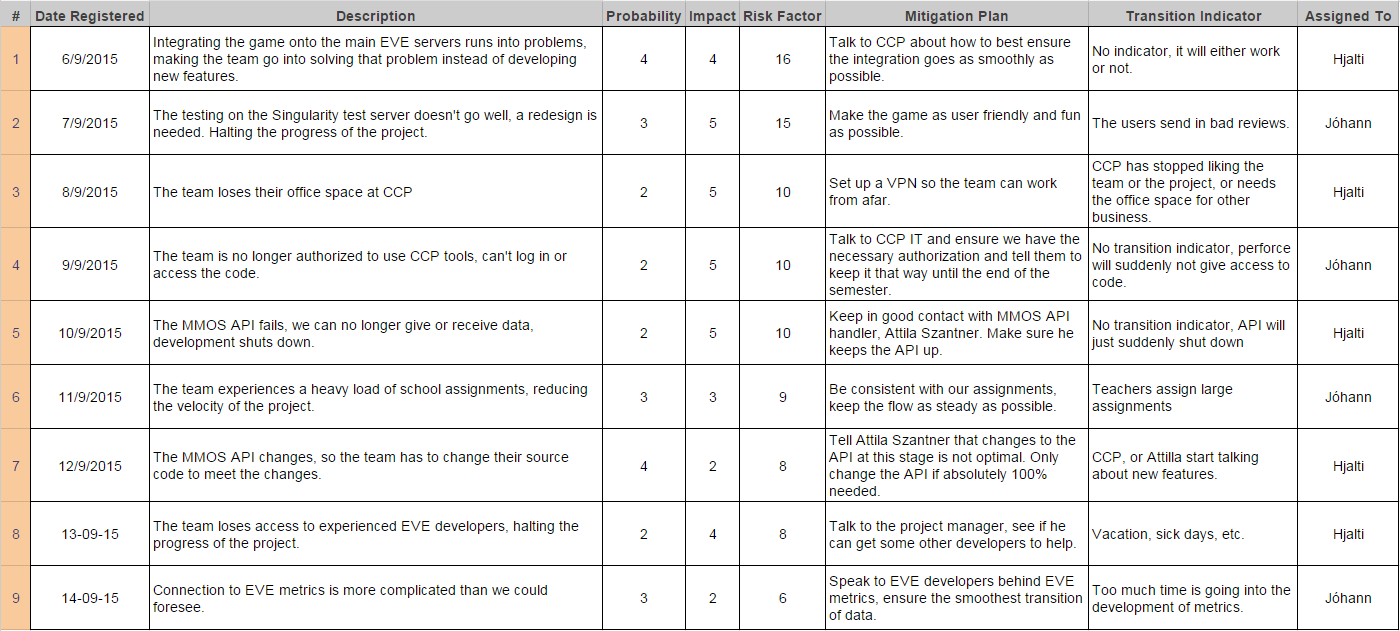
\includegraphics[scale=0.4]{risk.png}}
\caption{\label{fig:risk} Risk analysis for Project Discovery.}
\end{figure}
